\subsection{XBee Radios}

\frame{
 \frametitle{Why XBee Radios?}
  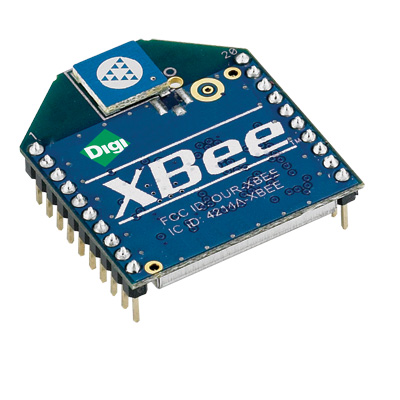
\includegraphics[scale=.16 ]{images/xBee.jpg}
 \begin{itemize}
  \item Small form factor (just larger than U.S. quarter)
  \item Low power consumption (\textasciitilde .1 W)
  \item Talk over ZigBee 802.15.4 standard
 \end{itemize}
}

\frame{
 \frametitle{ZigBee Specification}
 \begin{itemize}
  \item High level communications protocol
  \item Designed for low power digital radios
  \item Mesh network topology
  \item Network can expand on the fly
  \item 2.4GHz operating spectrum
 \end{itemize}
}

\frame{
 \frametitle{ZigBee Mesh and POW-R}
 \begin{itemize}
  \item One Coordinator per mesh
	\begin{itemize}
		\item Maintains mesh
		\item Receives transmissions from all router XBees
		\item Attached to POW-R server via Arduino
	\end{itemize}
  \item All Satellites have router XBees
  \item Router XBees "bounce" transmissions to Coordinator
 \end{itemize}
}